\documentclass{article}
\usepackage[T1]{fontenc}
\usepackage{lmodern}
\usepackage{graphicx}
\usepackage{amsmath,amssymb}
\usepackage[a4paper,margin=2cm]{geometry}
\usepackage[absolute,overlay]{textpos}
\setlength{\TPHorizModule}{1mm}
\setlength{\TPVertModule}{1mm}
\usepackage[indonesian]{babel}
\usepackage{hyperref}
\setlength{\emergencystretch}{2em}
% unit: Halaman 50

\begin{document}

% === Halaman 50 (llm) ===

\section*{Kode Program RC4 (dalam Bahasa C++)}

\vspace{172.26mm}

\begin{itemize}
    \item Enkripsi
\end{itemize}

\vspace{10mm}

% deskripsi: Screenshot cuplikan kode program C++ untuk implementasi enkripsi RC4 yang terbagi dalam dua kolom.
% bbox normalisasi: [0.0500, 0.3300, 0.9450, 0.9100]
\begin{textblock*}{187.95mm}(10.50mm,98.01mm)
\noindent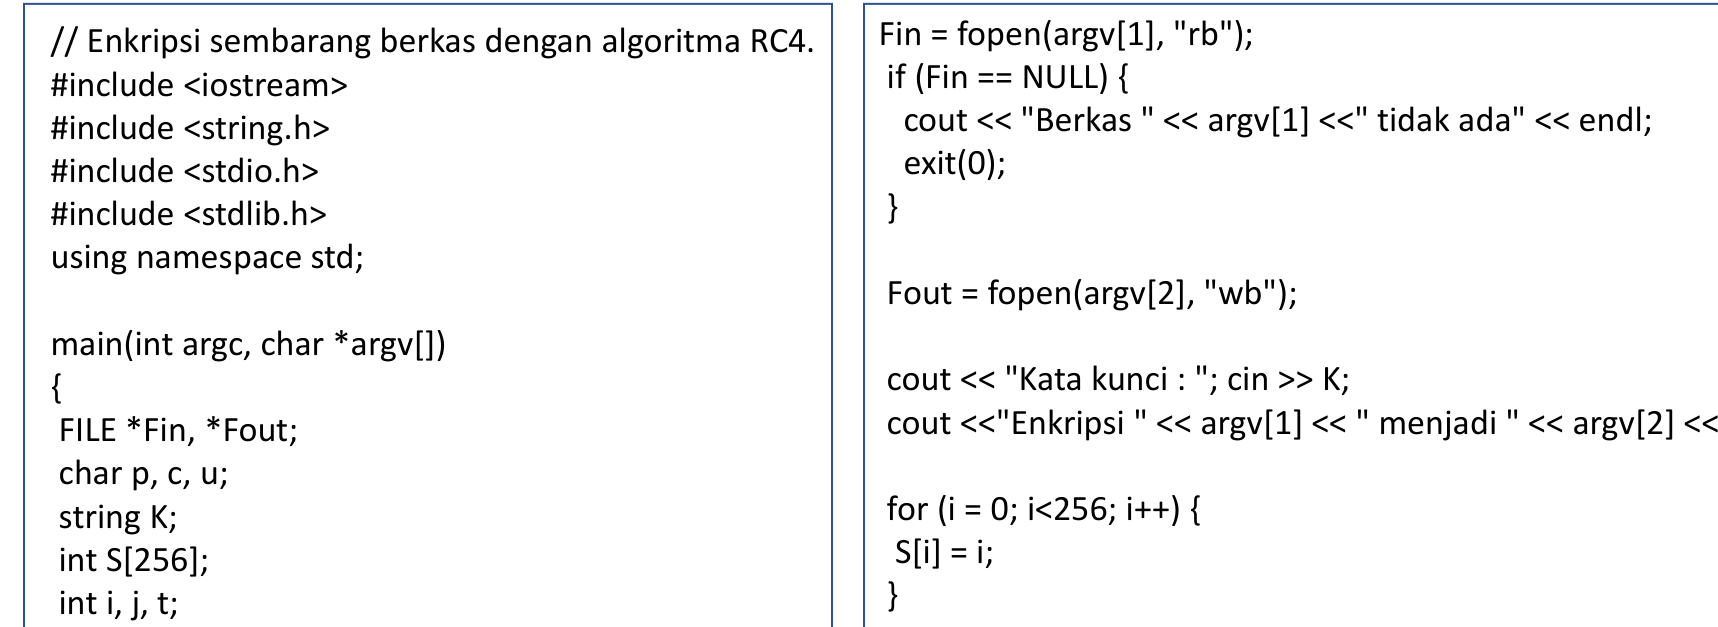
\includegraphics[width=187.95mm,height=172.26mm]{../../images/llm/page_050_img_01.png}%
\end{textblock*}

\end{document}
